\newif\ifshowsolutions
\showsolutionstrue
\documentclass{article}
\usepackage{listings}
\usepackage{amsmath}
%\usepackage{subfigure}
\usepackage{subfig}
\usepackage{amsthm}
\usepackage{amsmath}
\usepackage{amssymb}
\usepackage{graphicx}
\usepackage{mdwlist}
\usepackage[colorlinks=true]{hyperref}
\usepackage{geometry}
\usepackage{titlesec}
\geometry{margin=1in}
\geometry{headheight=2in}
\geometry{top=2in}
\usepackage{palatino}
\usepackage{mathrsfs}
\usepackage{fancyhdr}
\usepackage{paralist}
\usepackage{todonotes}
\setlength{\marginparwidth}{2.15cm}
\usepackage{tikz}
\usetikzlibrary{positioning,shapes,backgrounds}
\usepackage{float} % Place figures where you ACTUALLY want it
\usepackage{comment} % a hack to toggle sections
\usepackage{ifthen}
\usepackage{mdframed}
\usepackage{verbatim}
\usepackage[strings]{underscore}
\usepackage{listings}
\usepackage{bbm}
\rhead{}
\lhead{}

\renewcommand{\baselinestretch}{1.15}

% Shortcuts for commonly used operators
\newcommand{\E}{\mathbb{E}}
\newcommand{\Var}{\operatorname{Var}}
\newcommand{\Cov}{\operatorname{Cov}}
\newcommand{\Bias}{\operatorname{Bias}}
\DeclareMathOperator{\argmin}{arg\,min}
\DeclareMathOperator{\argmax}{arg\,max}

% do not number subsection and below
\setcounter{secnumdepth}{1}

% custom format subsection
\titleformat*{\subsection}{\large\bfseries}

% set up the \question shortcut
\newcounter{question}[section]
\newenvironment{question}[1][]
  {\refstepcounter{question}\par\addvspace{1em}\textbf{Question~\Alph{question}\!
    \ifthenelse{\equal{#1}{}}{}{ [#1 points]}: }}
    {\par\vspace{\baselineskip}}

\newcounter{subquestion}[question]
\newenvironment{subquestion}[1][]
  {\refstepcounter{subquestion}\par\medskip\textbf{\roman{subquestion}.\!
    \ifthenelse{\equal{#1}{}}{}{ [#1 points]:}} }
  {\par\addvspace{\baselineskip}}

\titlespacing\section{0pt}{12pt plus 2pt minus 2pt}{0pt plus 2pt minus 2pt}
\titlespacing\subsection{0pt}{12pt plus 4pt minus 2pt}{0pt plus 2pt minus 2pt}
\titlespacing\subsubsection{0pt}{12pt plus 4pt minus 2pt}{0pt plus 2pt minus 2pt}


\newenvironment{hint}[1][]
  {\begin{em}\textbf{Hint: }}{\end{em}}

\ifshowsolutions
  \newenvironment{solution}[1][]
    {\par\medskip \begin{mdframed}\textbf{Solution~\Alph{question}#1:} \begin{em}}
    {\end{em}\medskip\end{mdframed}\medskip}
  \newenvironment{subsolution}[1][]
    {\par\medskip \begin{mdframed}\textbf{Solution~\Alph{question}#1.\roman{subquestion}:} \begin{em}}
    {\end{em}\medskip\end{mdframed}\medskip}
\else
  \excludecomment{solution}
  \excludecomment{subsolution}
\fi



%%%%%%%%%%%%%%%%%%%%%%%%%%%%%%
% HEADER
%%%%%%%%%%%%%%%%%%%%%%%%%%%%%%

\chead{
  {\vbox{
      \vspace{2mm}
      \large
      Machine Learning \& Data Mining \hfill
      Caltech CS/CNS/EE 155 \hfill \\[1pt]
      Set 2\hfill
      January $19^\text{th}$, 2022 \\
    }
  }
}

\begin{document}
\pagestyle{fancy}



%%%%%%%%%%%%%%%%%%%%%%%%%%%%%%
% POLICIES
%%%%%%%%%%%%%%%%%%%%%%%%%%%%%%

\section*{Policies}
\begin{itemize}
	\item Due 9 PM PST, January $19^\text{th}$ on Gradescope. 
	\item You are free to collaborate on all of the problems, subject to the collaboration policy stated in the syllabus.
	\item In this course, we will be using Google Colab for code submissions. You will need a Google account.
\end{itemize}

\section*{Submission Instructions}
\begin{itemize}
	\item Submit your report as a single .pdf file to Gradescope (entry code 7426YK), under "Set 2 Report". 
	\item In the report, \textbf{include any images generated by your code} along with your answers to the questions.
	\item Submit your code by \textbf{sharing a link in your report} to your Google Colab notebook for each problem (see naming instructions below). Make sure to set sharing permissions to at least "Anyone with the link can view". \textbf{Links that can not be run by TAs will not be counted as turned in.} Check your links in an incognito window before submitting to be sure. 
	\item For instructions specifically pertaining to the Gradescope submission process, see \url{https://www.gradescope.com/get_started#student-submission}.
\end{itemize}

\section*{Google Colab Instructions}
For each notebook, you need to save a copy to your drive.
\begin{enumerate}
	\item Open the github preview of the notebook, and click the icon to open the colab preview.
	\item On the colab preview, go to File $\rightarrow$ Save a copy in Drive.
	\item Edit your file name to “lastname_firstname_set_problem”, e.g.”yue_yisong_set2_prob1.ipynb”
\end{enumerate}


%%%%%%%%%%%%%%%%%%%%%%%%%%%%%%
% PROBLEM 1
%%%%%%%%%%%%%%%%%%%%%%%%%%%%%%

\newpage
\section{Comparing Different Loss Functions [30 Points]}
\materials{lecture 3 \& 4}

We've discussed three loss functions for linear classification models so far:
\begin{itemize}
\item Squared loss: $L_\text{squared} = (1 - y\mathbf{w}^T\mathbf{x})^2$
\item Hinge loss: $L_\text{hinge} = \max(0, 1 - y\mathbf{w}^T\mathbf{x})$
\item Log loss: $L_\text{log} = \ln(1 + e^{-y\mathbf{w}^T\mathbf{x}})$
\end{itemize}
where $\mathbf{w} \in \mathbb{R}^n$ is a vector of the model parameters, $y \in \{-1,1\}$ is the class label for datapoint $\mathbf{x} \in \mathbb{R}^n$, and we're including a bias term in $\mathbf{x}$ and $\mathbf{w}$.  The model classifies points according to $\text{sign}(\mathbf{w}^T\mathbf{x})$.

Performing gradient descent on any of these loss functions will train a model to classify more points correctly, but the choice of loss function has a significant impact on the model that is learned.

\problem[3]
Squared loss is often a terrible choice of loss function to train on for classification problems.  Why?

\begin{solution}
 Generally, the squared loss heavily biases towards outliers. This is made worse for classification problems as the magnitude of the error will be $(1+|\mathbf{w}^T\mathbf{x}|)^2$. This will also bias against hypothesis with large $|\mathbf{w}^T\mathbf{x}|$.

 Furthermore, when the squared loss function is used as the objective function, the resulting function is non-convex, implying that we may not converge to the true minima when optimising the weights. 
\end{solution}

\problem[9]
A dataset is included with your problem set: \texttt{problem1data1.txt}. The first two columns represent $x_1, x_2$, and the last column represents the label, $y \in \{-1,+1\}$.

On this dataset, train both a logistic regression model and a ridge regression model to classify the points.  (In other words, on each dataset, train one linear classifier using $L_\text{log}$ as the loss, and another linear classifier using $L_\text{squared}$ as the loss.) For this problem, you should use the logistic regression and ridge regression implementations provided within scikit-learn 
(\href{http://scikit-learn.org/stable/modules/generated/sklearn.linear_model.LogisticRegression.html}{logistic regression documentation})
(\href{http://scikit-learn.org/stable/modules/generated/sklearn.linear_model.Ridge.html}{Ridge regression documentation})
instead of your own implementations. Use the default parameters for these classifiers except for setting the regularization parameters so that very little regularization is applied.

For each loss function/model, plot the data points as a scatter plot and overlay them with the decision boundary defined by the weights of the trained linear classifier.  Include both plots in your submission. The template notebook for this problem contains a helper function for producing plots given a trained classifier.

What differences do you see in the decision boundaries learned using the different loss functions? Provide a qualitative explanation for this behavior.

\begin{solution}
  Link: \url{https://colab.research.google.com/drive/1r7B7PM8hozxEy1vvvrfG8GUgO3Vchkly?usp=sharing}
  The figures below were obtained using ridge regression and logistic regression, respectively:
  \begin{figure}[H]
    \subfloat[]{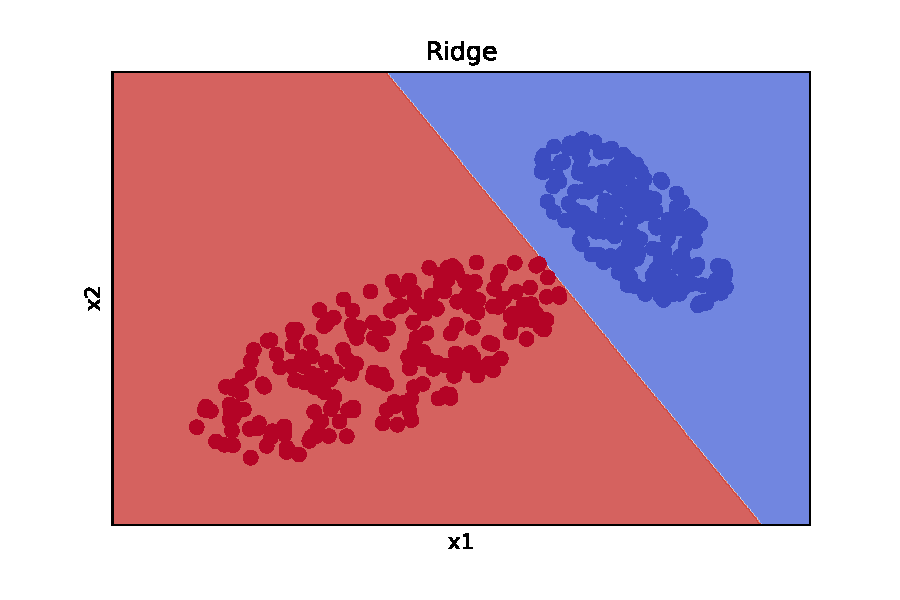
\includegraphics[width=0.49\textwidth]{ridge_P1.pdf}}
    \subfloat[]{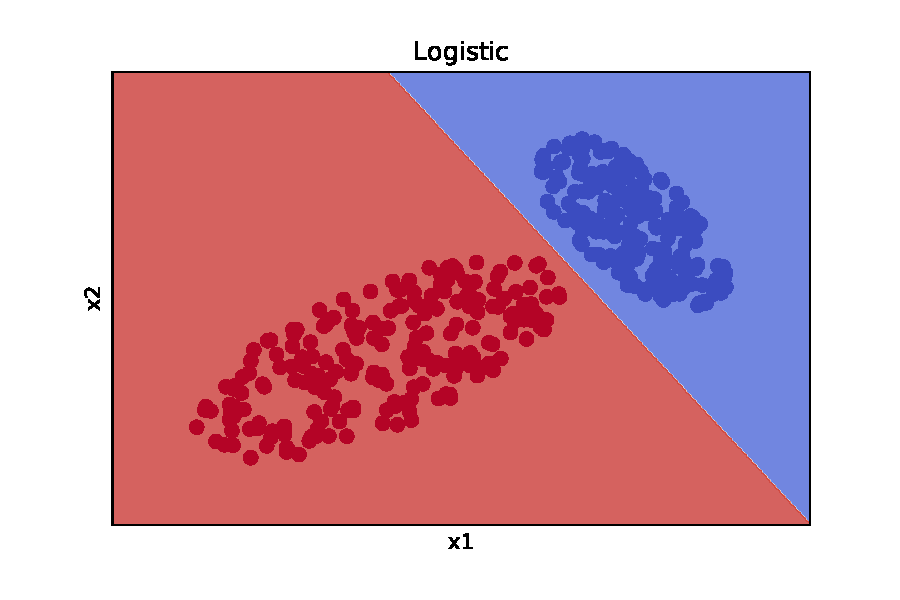
\includegraphics[width=0.49\textwidth]{logistic_P1.pdf}}
  \end{figure}
  In the case of ridge regression (or squared loss function), the boundary is very close to the boundary of the data points, in contrast to logistic regression. This is most likely because of the greater weighting of outliers in the case of the squared loss function, where these data points are more-strongly weighted when determining the parameters. This is not the case in logistic regression where the boundary is much more centered between the datasets.
\end{solution}

\problem[9]
Leaving squared loss behind, let's focus on log loss and hinge loss. Consider the set of points $S = \{(\frac{1}{2}, 3), (2, -2), (-3, 1)\}$ in 2D space, shown below, with labels $(1, 1, -1)$ respectively.

Given a linear model with weights $w_0 = 0, w_1 = 1, w_2 = 0$ (where $w_0$ corresponds to the bias term), compute the gradients $\nabla_{w}L_{\text{hinge}}$ and $\nabla_{w}L_{\text{log}}$ of the hinge loss and log loss, and calculate their values for each point in S.

\begin{center}
  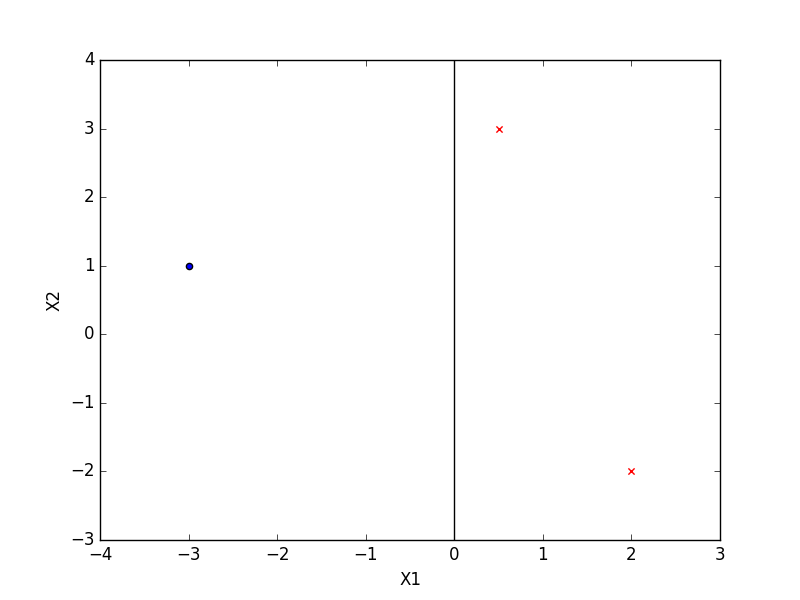
\includegraphics[width=.8\textwidth]{./images/SimpleDatasetWithDecisionBoundary.png}
\end{center}
\begin{small}
  The example dataset and decision boundary described above. Positive instances are
  represented by red x's, while negative instances appear as blue dots.
\end{small}

\begin{solution}
  The gradient of the Hinge loss function is given by:
  \begin{eqnarray*}
		\nabla_w L_{\text{Hinge}} = \begin{cases} 
		0 & y\textbf{w}^T\textbf{x} \geq 1 \\
		-y\textbf{x} & y\textbf{w}^T\textbf{x} < 1 \\ 
		\end{cases}\\
		\end{eqnarray*} 
  The gradient of the logistic loss function is given by:
  \begin{eqnarray*}
		\nabla_\textbf{w} L_{\text{log}} = \frac{-y\textbf{x}}{e^{\textbf{w}^{T}\textbf{x}y} + 1}
	\end{eqnarray*}
  As a result, the following values for the gradient at each data point was obtained:
  \begin{center}
    \begin{tabular}{|c| c|c|c|c|c|} 
      x$_1$ & x$_2$ & y & $\nabla_w$L$_{\text{Hinge}}$  & $\nabla_w$L$_{\text{log}}$ \\ 
      \hline
      0.5 & 3.0 & 1 & [-1,-0.5,-3] & [-0.378, -0.189, -1.133] \\ 
      2.0 & -2.0 & 1 & [0,0,0] & [-0.119, -0.238, 0.238] \\
      -3.0 & 1.0 & -1 & [0,0,0] & [0.047, -0.142, 0.047]\\
    \end{tabular}
  \end{center} 
\end{solution}

\problem[4]
Compare the gradients resulting from log loss to those resulting from hinge loss. When (if ever) will these gradients converge to 0? For a linearly separable dataset, is there any way to reduce or altogether eliminate training error without changing the decision boundary?

\begin{solution}
 In the case of the hinge loss function, it is possible for the gradient to reduce to 0 if all the data points are correctly classified (since at that point, $y\mathbf{w}^T\mathbf{x}\geq 1$). However, this does not appear to be the case for logistic regression as, even for points which are correctly classified, the gradient is non-zero. In fact, the only case for which the gradient will be 0, for a binary classification problem, will be when $\mathbf{x}=0$. It will, however, approach zero when $\exp{\mathbf{w}^T\mathbf{x}y}$ becomes infinitely large. 

 If a dataset is linearly separable, it should be possible to bring the training error to zero using a linear boundary. However, outliers will always be present and, as such, the training error can never truly be zero. For this reason, we include margins for our boundaries which aid in accounting for the presence of these outliers.
\end{solution}

\problem[5]
Based on your answer to the previous question, explain why for an SVM to be a ``maximum margin'' classifier, its learning objective must not be to minimize just $L_\text{hinge}$, but to minimize $L_\text{hinge} + \lambda\Vert w \Vert^2$ for some $\lambda > 0$.

(You don't need to prove that minimizing $L_\text{hinge} + \lambda\Vert w \Vert^2$ results in a maximum margin classifier; just show that the additional penalty term addresses the issues of minimizing just $L_\text{hinge}$.)

\begin{solution}
 The hinge loss function, as shown previously, will converge once all points have been classified correctly. However, this does mean that some points may lie directly on the boundary, leaving no room for margin of error. This beats the purposes of SVM being `maximum margin' classifier. 

 The addition of the penatly prevents the algorithm from converging to the first weights which minimise the hinge loss function. By tuning the $\lambda$ parameter, we can force the classifier to converge to a solution with larger margins, in order to avoid having points on the boundary of our classifier.
\end{solution}

\newpage
\section{Effects of Regularization}
\textit{Relevant materials: Lecture 3 \& 4}

For this problem, you are required to implement everything yourself and submit code (i.e. don't use scikit-learn but numpy is fine).
\indent\problem[4] 
In order to prevent over-fitting in the least-squares linear regression problem, we add a regularization penalty term.
Can adding the penalty term decrease the training (in-sample) error?
Will adding a penalty term always decrease the out-of-sample errors?
Please justify your answers. Think about the case when there is over-fitting while training the model.

\begin{solution}
 Generally, adding a penalty term will not improve the in-sample error as, by constraining the weights, we are reducing the range of weights the classifiers can choose. Either the weights will be within the constrained space (and match the unconstrained solution) or it will lie on the boundary of the constraint. We do, however, expect it to decrease the out-of-sample error. By constraining the classifier, we are making it less susceptible to noise and random errors which typically lead to overfitting. By avoiding overfitting, we (hopefully) end up with a model that more-accurately characterises the underlying behaviour of the dataset, thus yielding a more-accurate model. However, if regularisation is overdone, we can actually worsen the solution as we will miss-out on some of the underlying behaviour of the dataset.
\end{solution}

\problem[4]
$\ell_1$ regularization is sometimes favored over $\ell_2$ regularization due to its ability to generate a sparse $w$ (more zero weights).
In fact, $\ell_0$ regularization (using $\ell_0$ norm instead of $\ell_1$ or $\ell_2$ norm) can generate an even sparser $w$, which seems favorable in high-dimensional problems.
However, it is rarely used.  Why?

\begin{solution}
 $\ell_0$ regularization effectively constrains the number of weights. Whilst this is effectively what $\ell_1$ and $\ell_2$ regularisation are doing, this isn't as direct a constraint. Furthermore, $\ell_0$ regularization is non-convex and non-continuous, making it very difficult to optimise for as we will not be able to obtain simple derivatives for the loss function.
\end{solution}

\subsection{Implementation of \texorpdfstring{$\ell_2$}{L2} regularization:}

We are going to experiment with regression for the Red Wine Quality Rating data set. The data set is uploaded on the course website, and you can read more about it here: \url{https://archive.ics.uci.edu/ml/datasets/Wine}. The data relates 13 different factors (last 13 columns) to wine type (the first column). Each column of data represents a different factor, and they are all continuous features. Note that the original data set has three classes, but one was removed to make this a binary classification problem.

Download the data for training and validation from the assignments data folder.
There are two training sets, wine\_training1.txt (100 data points) and wine\_training2.txt (a proper subset of wine\_training1.txt containing only 40 data points), and one test set, wine\_validation.txt (30 data points). You will use the wine\_validation.txt dataset to evaluate your models.

We will train a \emph{$\ell_2$-regularized logistic regression} model on this data. Recall that the unregularized logistic error (a.k.a. log loss) is
\[E = -\sum_{i=1}^{N}\log(p(y_i | \mathbf{x}_i))\]

where $p(y_i = -1 | \mathbf{x}_i)$ is
\[\frac{1}{1 + e^{\mathbf{w}^T\mathbf{x}_i}}\]

and $p(y_i = 1 | \mathbf{x}_i)$ is
\[\frac{1}{1 + e^{-\mathbf{w}^T\mathbf{x}_i}},\]
where as usual we assume that all $\mathbf{x}_i$ contain a bias term.
The $\ell_2$-regularized logistic error is 
\begin{align*}
  E &= -\sum_{i=1}^{N}\log(p(y_i | \mathbf{x}_i)) + \lambda\mathbf{w}^T\mathbf{w} \\
    &= -\sum_{i=1}^{N} \log \left( \frac{1}{1 + e^{-y_i\mathbf{w}^T\mathbf{x}_i}} \right) + \lambda\mathbf{w}^T\mathbf{w} \\
    &= -\sum_{i=1}^{N} \left(\log \left( \frac{1}{1 + e^{-y_i\mathbf{w}^T\mathbf{x}_i}} \right) - \frac{\lambda}{N}\mathbf{w}^T\mathbf{w}\right).
\end{align*}
Implement SGD to train a model that minimizes the $\ell_2$-regularized logistic error, i.e. train an $\ell_2$-regularized logistic regression model.  Train the model with 15 different values of $\lambda$ starting with $\lambda_0 = 0.00001$ and increasing by a factor of 5, i.e. $$\lambda_0 = 0.00001, \lambda_1 = 0.00005, \lambda_2 = 0.00025, ..., \lambda_{14} = 61,035.15625.$$
\par

Some important notes: Terminate the SGD process after 20,000 epochs, where each epoch performs one SGD iteration for each point in the training dataset. You should shuffle the order of the points before each epoch such that you go through the points in a random order (hint: use \texttt{numpy.random.permutation}). Use a learning rate of $5 \times 10^{-4}$, and initialize your weights to small random numbers. 

You may run into numerical instability issues (overflow or underflow). One way to deal with these issues is by normalizing the input data $X$. Given the column for the $j$th feature, $X_{:,j}$, you can normalize it by setting $X_{ij} = \frac{X_{ij} - \overline{X_{:,j}} }{\sigma(X_{:,j})}$ where $\sigma(X_{:,j})$ is the standard deviation of the $j$th column's entries, and $\overline{X_{:,j}}$ is the mean of the $j$th column's entries. Normalization may change the optimal choice of $\lambda$; the $\lambda$ range given above corresponds to data that has been normalized in this manner. If you treat the input data differently, simply plot enough choices of $\lambda$ to see any trends.

\problem[16]
Do the following for both training data sets (wine\_training1.txt and wine\_training2.txt) and attach your plots in the homework submission (use a log-scale on the horizontal axis):

\subproblem Plot the average training error ($E_\text{in}$) versus different $\lambda$s.

\subproblem Plot the average test error ($E_\text{out}$) versus different $\lambda$s using wine\_validation.txt as the test set.

\subproblem Plot the $\ell_2$ norm of $\mathbf{w}$ versus different $\lambda$s. \medskip

 You should end up with three plots, with two series (one for wine\_training1.txt and one for wine\_training2.txt) on each plot. Note that the $E_\text{in}$ and $E_\text{out}$ values you plot should not include the regularization penalty --- the penalty is only included when performing gradient descent.

\begin{solution}
  Link: \url{https://colab.research.google.com/drive/1hQdY20GGnvcu_0edQYeQMpQwINQM7_MC?usp=sharing}
  The following figures were generated:
  \begin{figure}[H]
    \subfloat[]{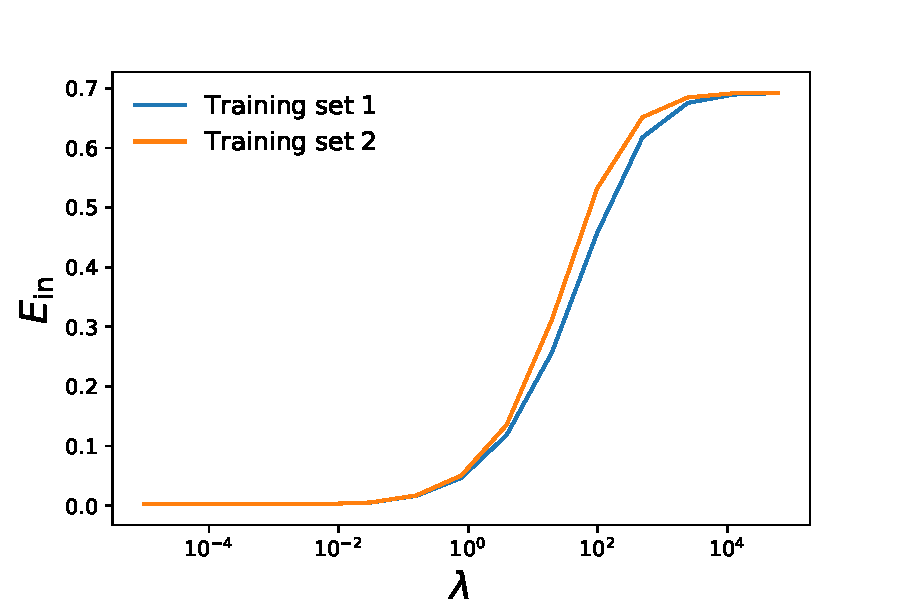
\includegraphics[width=0.5\textwidth]{E_in_2.pdf}}\\
    \subfloat[]{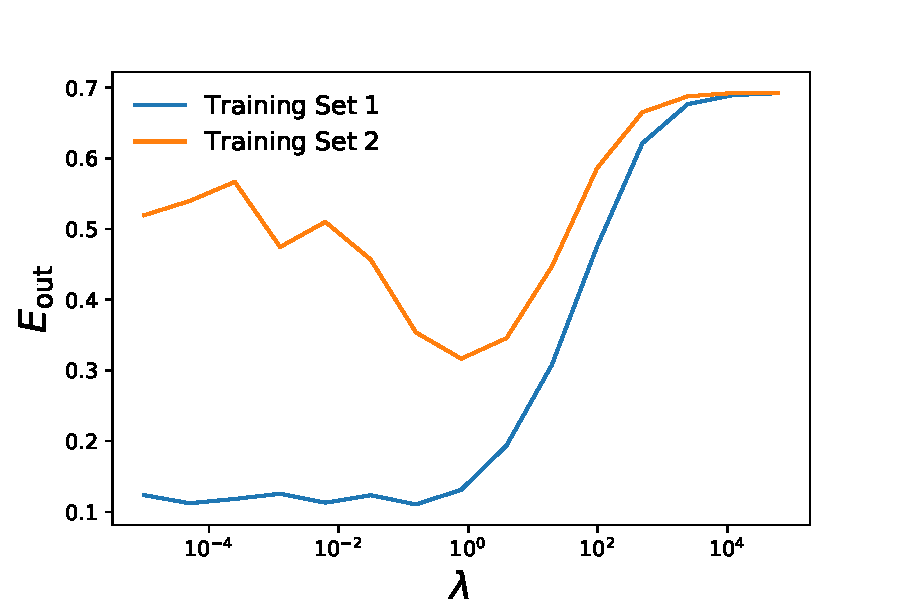
\includegraphics[width=0.5\textwidth]{E_out_2.pdf}}\\
    \subfloat[]{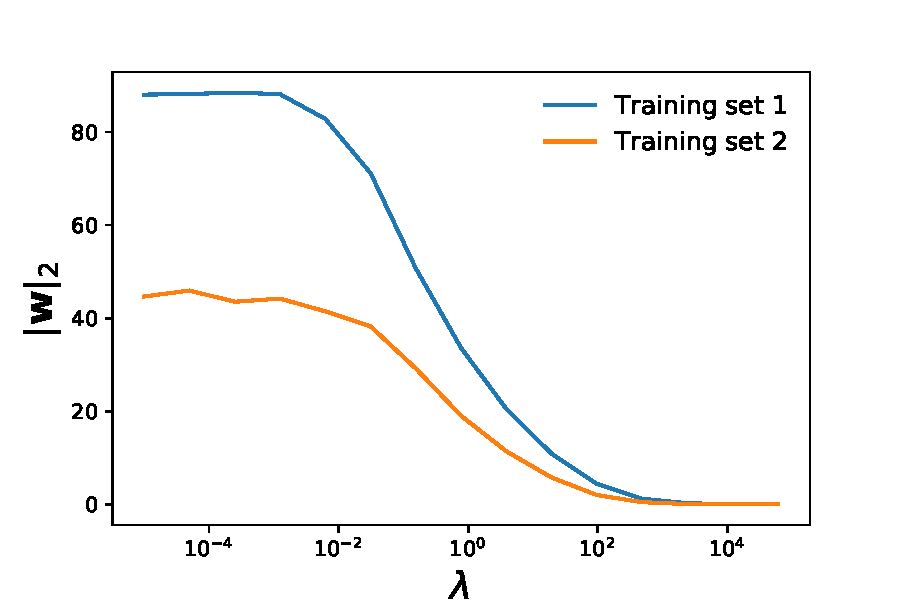
\includegraphics[width=0.5\textwidth]{l2norm_2.pdf}}
  \end{figure}
\end{solution}

\problem[4]
Given that the data in wine\_training2.txt is a subset of the data in wine\_training1.txt, compare errors (training and test) resulting from training with wine\_training1.txt (100 data points) versus wine\_training2.txt (40 data points). Briefly explain the differences.

\begin{solution}
 In terms of training error, $E_\text{in}$ is practically identical for both data sets. This is not too surprising as, if training set 2 is a representative subset of training set 1, they will capture the same behaviour, thus yield very similar errors. At low $\lambda$, training set 2 obtains slightly lower errors than training set 1, most likely because the same number of parameters have fewer data points to fit and, given they aren't constrained, they are able to overfit. However, at larger $\lambda$, where the parameters are more-constrained, training set 1 has the smaller error, primarily because training set 2 has fewer data points to fit the limited number of parameters.

 However, in the testing error, there are significant differences, where training set 2 yields greater errors than training set 1. At low $\lambda$, we observe overfitting as, with unconstrained parameters, they can account for the noise in the smaller data set, thus yield a greater $E_\text{out}$. We observe a minima in $E_\text{out}$ for both data sets, highlighting that we've limited overfitting for these data sets. However, beyond this minima, as we further constrain the parameters, they are less able to correctly characterise the underlying behaviour in the dataset, thus resulting in a greater, and similar, $E_\text{out}$.
\end{solution}

\problem[4]
Briefly explain the qualitative behavior (i.e. over-fitting and under-fitting) of the training and test errors with different $\lambda$s while training with data in wine\_training1.txt.

\begin{solution}
 As explained previously, at low $\lambda$, we are observing some slight overfitting of training set 1, highlighted by the decrease in $E_\text{out}$ with increasing $\lambda$. At around $\lambda=5\times 10^{-1}$, we observe a minimum in $E_\text{out}$, indicating the point where we've limited overfitting. Beyond this point, we begin over-constraining the weights, leading to under-fitting and significant increases in $E_\text{out}$.
\end{solution}

\problem[4]
Briefly explain the qualitative behavior of the $\ell_2$ norm of $\textbf{w}$ with different $\lambda$s while training with the data in wine\_training1.txt.

\begin{solution}
   Unsurprisingly, we observe a decrease in $\|\mathbf{w}\|_2$ with increasing $\lambda$. This is primarily because, with increasing $\lambda$, we are constraining the value of $\|\mathbf{w}\|_2^2$ directly. Thus, with increasing $\lambda$, $\|\mathbf{w}\|_2$ will always decrease.
\end{solution}

\problem[4]
If the model were trained with wine\_training2.txt, which $\lambda$ would you choose to train your final model? Why?

\begin{solution}
  The minimum in $E_\text{out}$ occurs at approximately $\lambda=10^{0}$, thus highlighting this is the point where we've limited the extent of overfitting and we have obtained the `best' weights for this data set. We can then use a testing set to evaluate the performance of these parameters.
\end{solution}

% Question 2
\newpage
\section{Lasso (\texorpdfstring{$\ell_1$}{L1}) vs. Ridge (\texorpdfstring{$\ell_2$}{L2}) Regularization}
\textit{Relevant materials: Lecture 3}

For this problem, you may use the scikit-learn (or other Python package) implementation of Lasso and Ridge regression --- you don't have to code it yourself.

The two most commonly-used regularized regression models are Lasso ($\ell_1$) regression and Ridge ($\ell_2$) regression.
Although both enforce ``simplicity'' in the models they learn, only Lasso regression results in sparse weight vectors.
This problem compares the effect of the two methods on the learned model parameters.

\problem[12] 
The tab-delimited file problem3data.txt on the course website contains 1000 9-dimensional datapoints.  The first 9 columns contain $x_1,\ldots,x_9$, and the last column contains the target value $y$.

\subproblem
Train a linear regression model on the problem3data.txt data with Lasso regularization for regularization strengths $\alpha$ in the vector given by \texttt{numpy.linspace(0.01, 3, 30)}.
On a single plot, plot each of the model weights $w_1, ..., w_9$ (ignore the bias/intercept) as a function of $\alpha$.

\subproblem
Repeat \textbf{i.} with Ridge regression, and this time using regularization strengths $\alpha \in \{1, 2, 3, \ldots, 1e4\}$.


\subproblem
As the regularization parameter increases, what happens to the number of model weights that are exactly zero with Lasso regression?
What happens to the number of model weights that are exactly zero with Ridge regression?

\medskip
\lstset{
  basicstyle=\small\ttfamily,
  breaklines=true,
  columns=fullflexible
}

\begin{solution}
  Link: \url{https://colab.research.google.com/drive/1f_Ao2h1KfK2E4zRx0rvHbgUGKPDk9Wey?usp=sharing}
  \begin{enumerate}
    \item The following plot was generated:
    \begin{figure}[H]
      \subfloat[]{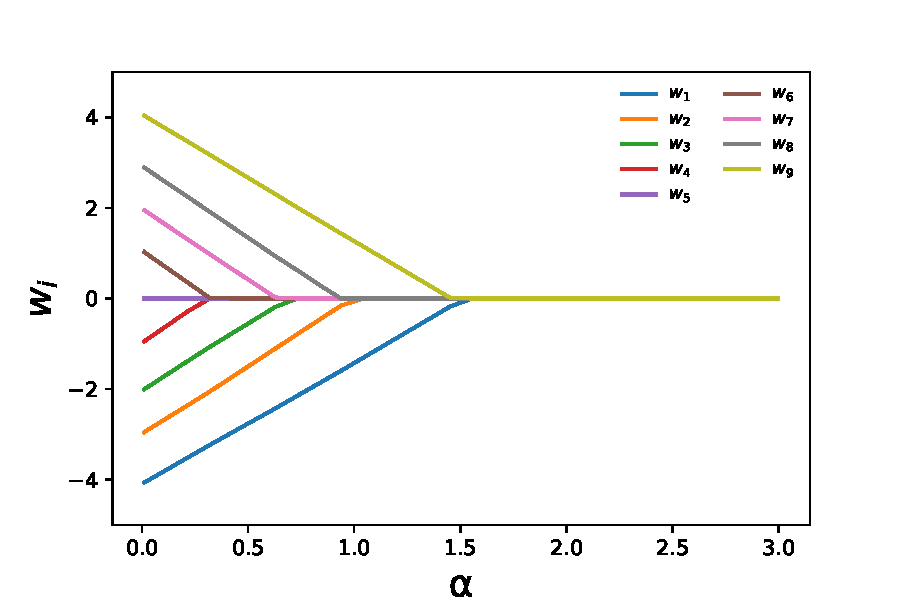
\includegraphics[width=0.5\textwidth]{lasso_3.pdf}}
    \end{figure}
    \item The following plot was generated:
    \begin{figure}[H]
      \subfloat[]{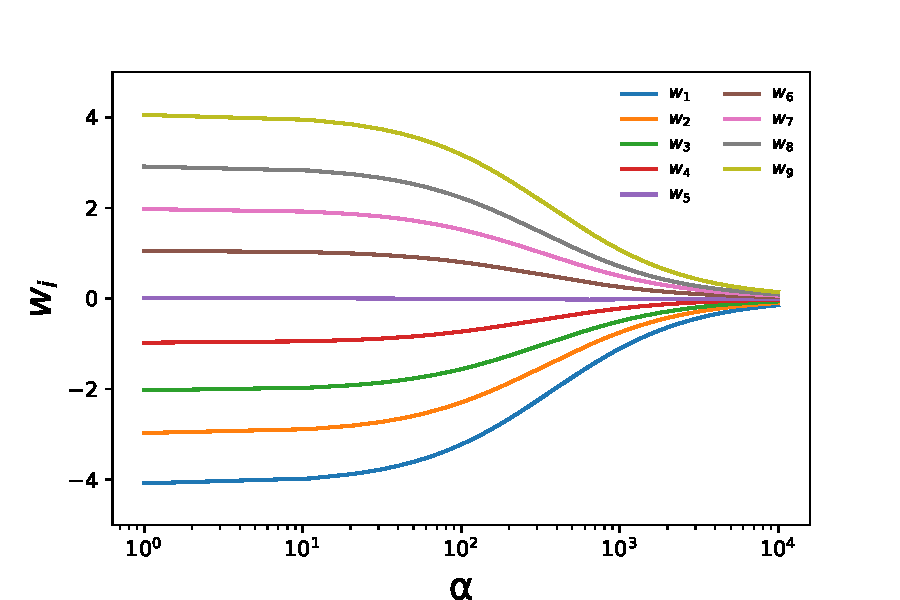
\includegraphics[width=0.5\textwidth]{ridge_3.pdf}}
    \end{figure}
    \item Within Lasso, as it is an $\ell_1$ regularisation, as the hyperparameter increases, the weights eventually get set to 0. One can see this above where, one by one, the weights get set to zero, the order of which depends on their initial magnitude. By $\alpha=1.6$, all weights are set to 0. 
    
    On the other hand, in ridge regression, although the weights approach 0, they do so asymtotically. Even in the case of $w_5$, its value is small but non-zero. This is the nature of $\ell_2$ regularisation.
  \end{enumerate}
\end{solution}

\problem[9]

\subproblem
In the case of 1-dimensional data, Lasso regression admits a closed-form solution.
Given a dataset containing $N$ datapoints, each with $d = 1$ feature, solve for
\[\underset{w}{\argmin} \Vert\mathbf{y} - \mathbf{x}w\Vert^2 + \lambda\Vert w\Vert_1,
\]
where $\mathbf{x} \in \mathbb{R}^{N}$ is the vector of datapoints and $\mathbf{y} \in \mathbb{R}^N$ is the  vector of all output values corresponding to these datapoints. Just consider the case where $d = 1$, $\lambda \geq 0$, and the weight $w$ is a scalar.

This is linear regression with Lasso regularization.

\begin{subsolution}
 \begin{equation}
   \partial_w(\Vert\mathbf{y} - \mathbf{x}w\Vert^2 + \lambda\Vert w\Vert_1) = -2\mathbf{x}^T\mathbf{y}+2\mathbf{x}^T\mathbf{x}w+\lambda \frac{w}{|w|}= 0
 \end{equation}
 \begin{equation}
  w = \frac{\mathbf{x}^T\mathbf{y}}{\mathbf{x}^T\mathbf{x}}-\frac{\lambda}{2\mathbf{x}^T\mathbf{x}}\frac{w}{|w|}
\end{equation}
\end{subsolution}

\subproblem
In this question, we continue to consider Lasso regularization in 1-dimension. Now, suppose that $w \neq 0$ when $\lambda = 0$. Does there exist a value for $\lambda$ such that $w = 0$? If so, what is the smallest such value?

\begin{subsolution}
  The above function is undefined at $w=0$. Thus taking the limit $w\rightarrow 0^+$:
  \begin{equation}
    0 = \frac{\mathbf{x}^T\mathbf{y}}{\mathbf{x}^T\mathbf{x}}-\frac{\lambda}{2\mathbf{x}^T\mathbf{x}}
  \end{equation}
  \begin{equation}
    \lim_{w\rightarrow 0^+}\lambda = 2|\mathbf{x}^T\mathbf{y}|
  \end{equation}
  An identical solution is obtained when we approach $0^-$.
\end{subsolution}

\problem[9]
\subproblem
Given a dataset containing $N$ datapoints each with $d$ features, solve for
\[\underset{\mathbf{w}}{\argmin} \Vert\mathbf{y} - \mathbf{X}\mathbf{w}\Vert^2 + \lambda\Vert\mathbf{w}\Vert_2^2
\]
where $\mathbf{X} \in \mathbb{R}^{N \times d}$ is the matrix of datapoints and $\mathbf{y} \in \mathbb{R}^N$ is the  vector of all output values for these datapoints. Do so for arbitrary $d$ and $\lambda \geq 0$.

This is linear regression with Ridge regularization.

\begin{subsolution}
  \begin{align}
    \partial_w &\left( \|\textbf{y} - \textbf{X}^{T}\textbf{w}\|^2 + \lambda\|\textbf{w}\|_2^2\right) \\
    &= -2\textbf{X}^T (\textbf{y} - \textbf{X}^{T}\textbf{w}) + 2\lambda\textbf{w} = 0 \\
  \textbf{w} &= \textbf{X}^T\textbf{y}(\lambda I + \textbf{X}^T\textbf{X})^{-1}
    \end{align} 
\end{subsolution}

\subproblem In this question, we consider Ridge regularization in 1-dimension. Suppose that $w \neq 0$ when $\lambda = 0$. Does there exist a value for $\lambda > 0$ such that $w = 0$? If so, what is the smallest such value?

\begin{subsolution}
 There is no $\lambda$ for which $w=0$ .
\end{subsolution}

\end{document}

%%% Local Variables:
%%% mode: latex
%%% TeX-master: t
%%% End: